%!TEX root = chi14grammatical.tex

\begin{figure*}
	\begin{subfigure} {1.3\columnwidth}
			\centering
	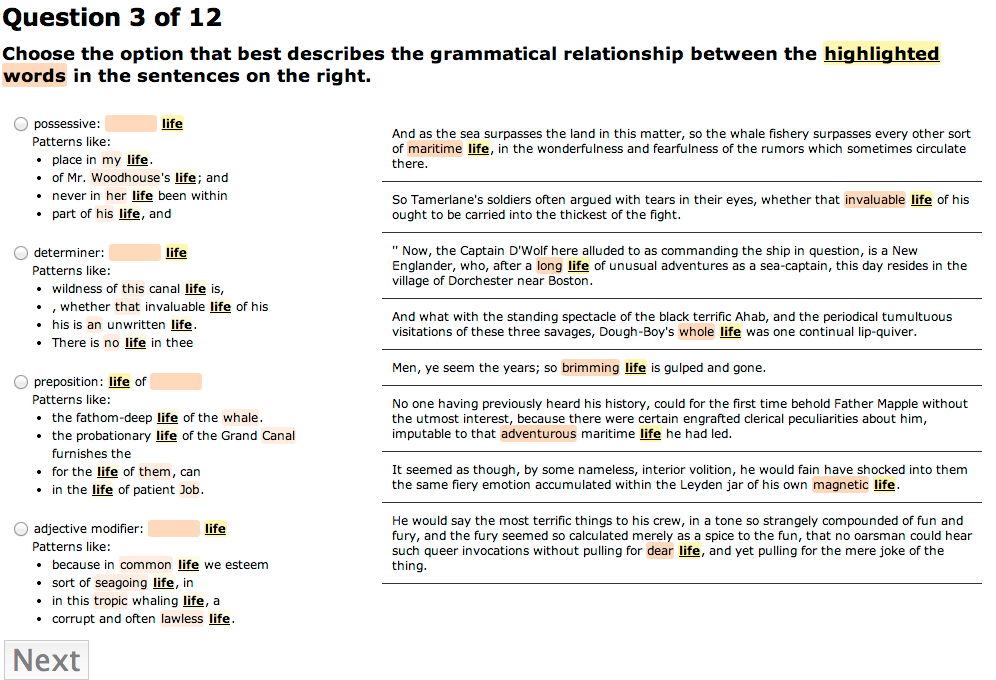
\includegraphics[width=1.2\columnwidth]{fig/task}
	\caption{\label{fig:task} An example of an identification task in the \emph{phrases} condition for the relationship \code{amod(life, \_\_\_)} (where different adjectives modify the noun `life'). The correct answer is `adjective modifier' (4th option), and the remaining 3 options are distractors.}
	\end{subfigure}
	\qquad\qquad\qquad
	\begin{subfigure}{0.7\columnwidth}
		\begin{subfigure}{0.7\columnwidth}
				\centering
		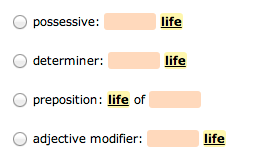
\includegraphics[width=0.9\columnwidth]{fig/baseline-choices}
	    \caption {The same options as they appear in the \emph{baseline} condition \label{fig:baseline-choices}}
	    \end{subfigure}


	    \begin{subfigure}{0.7\columnwidth}
	    	\centering
	    	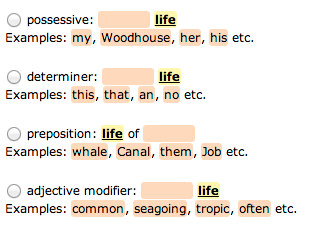
\includegraphics[width=0.9\columnwidth]{fig/words-choices}
	        \caption {The same options as they appear in the \emph{words} condition \label{fig:words-choices}}
	    \end{subfigure}
	\end{subfigure}
\caption{\label{fig:choices} The way the choices appeared in the three experiment conditions.}
\end{figure*}

Our goal was to find out whether showing examples improves the recognizability of grammatical relations. We tested two types of examples: a list of matching words and a list of matching phrases. Words are explicitly visible in the text, but phrases provides contextual information that helps determine the relationship, such as the part of speech, the relative ordering, and any accompanying words.

Our hypothesis was the following:
\begin{quote}
	H1. Grammatical relations can be made more recognizable by showing examples of words or phrases that match.
\end{quote}

To test it, we gave participants a series of identification tasks. In each task, participants were shown list of 8 sentences, each containing a particular relationship between highlighted words. They were asked to identify which relationship it was from list of 4 choices

We displayed the choices in 3 different ways (Figure \ref{fig:choices}). The \strong{baseline} presentation was a short label using linguistic terminology (Figure \ref{fig:baseline-choices}), the \strong{words} presentation was the short label accompanied by a list of words that matched (Figure \ref{fig:words-choices}), and the \strong{phrases} presentation was the short label accompanied by a list of phrases in which that relationship surfaced (Figure \ref{fig:task}).

We used a between-subjects design. The tasks were presented in the same order, and the choices were also presented in the same order: the only variation between participants was the way in which those choices were displayed. We measured whether participants in the \strong{words} or \strong{phrases} condition identified relationships more accurately than participants in the \strong{baseline} condition.

To avoid the possibility of participants guessing the right answer by pattern-matching, we ensured that there was no overlap between the list of sentences shown, and the examples shown in the choices as words or phrases.

The tasks were all generated using the Stanford Parser on the text of \emph{Moby Dick} by Herman Melville.  We tested the 12 most common grammatical relationships in the novel, which fell into the two categories below.

\squishlist
\item Clausal or long-distance relations:
	\squishlist
		\item \strong{advcl} Adverbial clause: \emph{  she \textbf{said} it while \textbf{smiling}}
		\item  \strong{xcomp} Open clausal complement:  \emph{I \textbf{learned} to \textbf{sing} }
		\item  \strong{ccomp} Clausal complement:  \emph{ I \textbf{thought} that I \textbf{knew} it}
		\item  \strong{rcmod} Relative clause modifier:  \emph{the \textbf{cat}, which we \textbf{rescued}, slept }
	\squishend
\item Other relations:
		\squishlist
			\item \strong{nsubj} Subject of verb: \emph{\textbf{he} \textbf{threw} the ball}
			\item \strong{dobj} Object of verb:  \emph{ he \textbf{threw} the \textbf{ball}}
			\item \strong{amod} Adjective modifier \emph{\textbf{red} \textbf{ball}}
			\item \strong{prep\_in}  Preposition (in): \emph{ the \textbf{water} in the \textbf{bucket}}
			\item \strong{prep\_of}	Preposition (of):  \emph{ the \textbf{piece} of \textbf{cheese}}
			\item \strong{conj\_and}  Conjunction (and)  \emph{ \textbf{mind} and \textbf{body}}
		\item\strong{advmod} Adverbial modifier: \emph{  she \textbf{said} it \textbf{slowly}}
		\item \strong{nn} Noun compound:  \emph{ \textbf{Mr.}  \textbf{Brown}}
		\squishend
\squishend

We tested each of the above relations 4 times, with 2 different words in each role. For example, the verb-subject relation \code{nsubj} was tested in the following four forms:
\squishlist
	\item \code{nsubj(Ahab, \_\_\_)}:  the sentences each contained `Ahab', highlighted in yellow, as the subject of different verbs highlighted in pink.
	\item \code{nsubj(captain, \_\_\_)}

	\item \code{nsubj(\_\_\_, said)}: the sentences all contained the verb `said', highlighted in yellow, but with different subjects, highlighted in pink.
	\item \code{nsubj(\_\_\_, stood)}
\squishend

To maximize coverage, yet keep the total task time reasonable (around 7 or 8 minutes), we divided the relations above into 4 task sets of 3 relations each. Each relation was tested with 4 different words, making a total of 12 tasks per participant.

\subsection{Participants}
We chose Amazon's Mechanical Turk crowdsourcing platform as a source of study participants because syntactic search is relevant to many fields outside linguistics and language study and we wanted to avoid having any specific backgrounds overrepresented. There were 400 participants, distributed randomly over the 4 task sets and the 3 presentations.

Participants were paid 50c (U.S.) for completing the task, with an additional 50c bonus if they correctly identified 10 or more of the 12 relationships. They were informed of the possibility of the bonus before starting the task.

As is difficult to ensure the quality of effort from participants from Mechanical Turk, we included a multiple-choice screening question, `What is the third word of this sentence?"  Those that answered incorrectly were eliminated.


\subsection{Results}
\begin{figure}
\centering
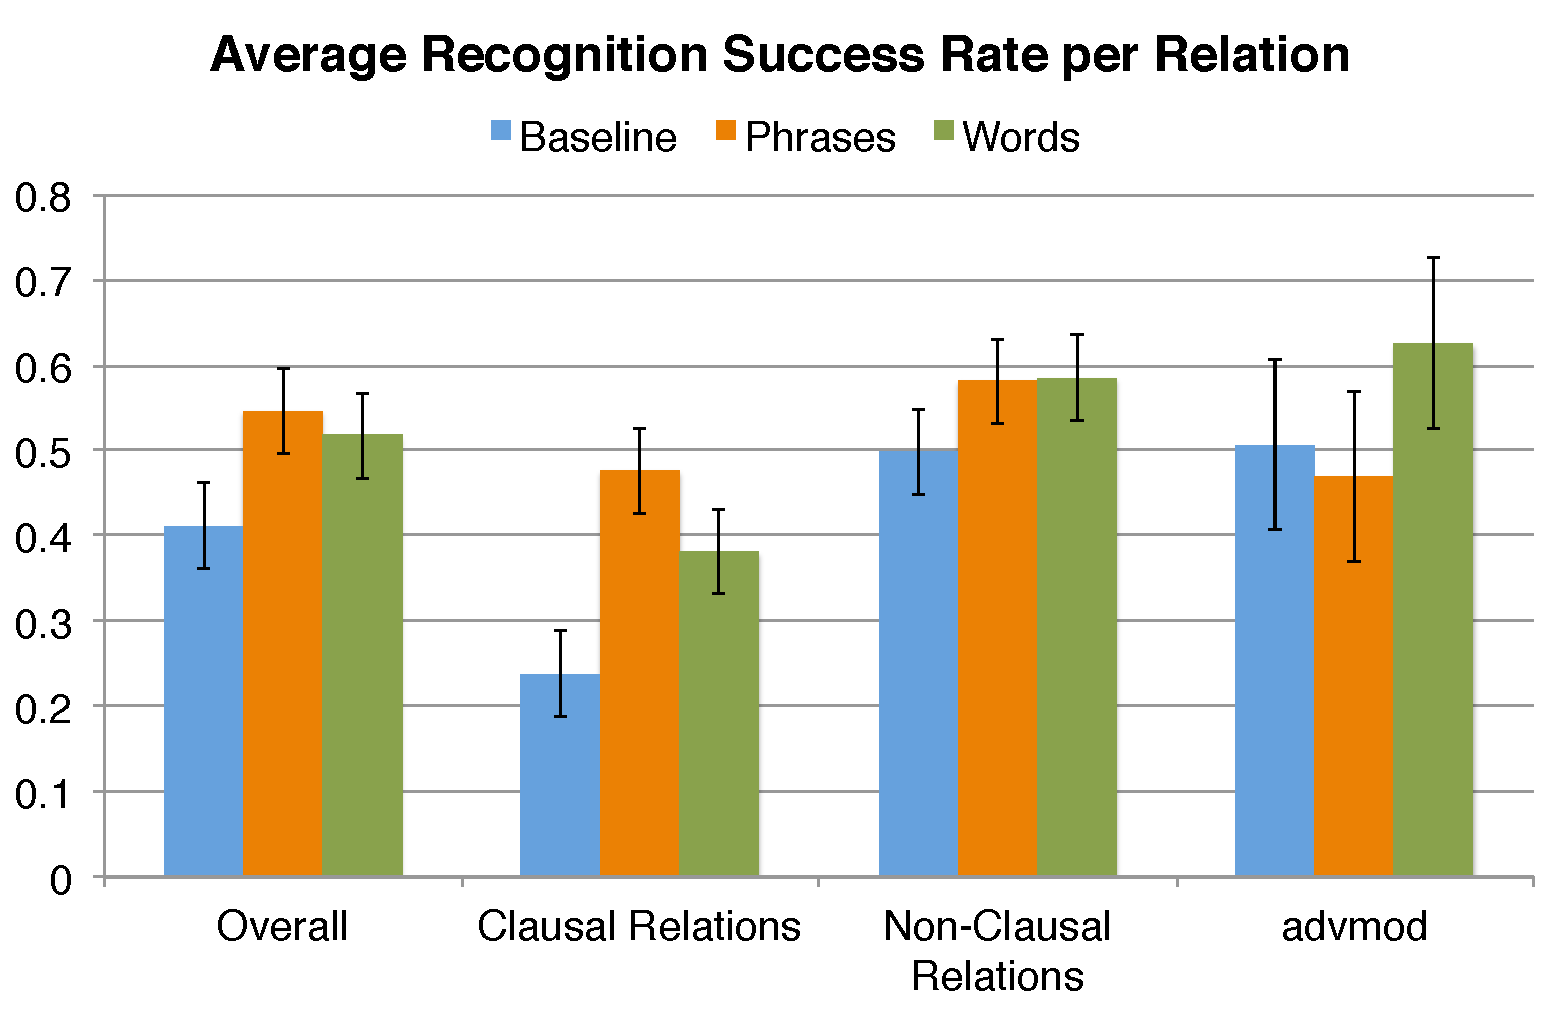
\includegraphics[width=\columnwidth]{fig/results}
\caption{\label{fig:results}Recognition rates per relation under the different experiment conditions.}
\end{figure}
Our results (Figure \ref{fig:results}) confirm H1. Examples improve the recognizability of grammatical relations. Participants in the \strong{baseline} condition were significantly worse at identifying the relations than participants in conditions that showed examples (\strong{phrases} and \strong{words}).  The average success rate (where success means that the participant correctly identified the relation) in the \strong{baseline} condition was $41\%$, which is significantly\footnote{Using the Wilcoxson signed-rank test, an alternative to the standard T-test that does not assume samples are normally distributed.} less accurate than in the two example-showing conditions: \strong{words}: $52\%, (p = 0.00019)$, and \strong{phrases} condition : $55\%, (p = 0.00013)$.

The difference between the two types of examples,  \strong{phrases} and \strong{words},  was not significant overall, but the data revealed an interesting fact when they were compared across the different types  of relations (Figure \ref{fig:results}). In all cases, the baseline performs worse that an example-showing presentation. However, the three different categories of relations behaved very differently with respect to whether phrases or words was better.

For the clausal relations, which operate over longer distances in sentences, the data confirmed what one might intuitively expect. Phrases, which show the usage context, significantly improved recognizability compared to the list of words or the baseline labels. The average success rate is 48\% for \strong{phrases}, which is significantly more than \strong{words}: 38\%, (p = 0.017), or \strong{baseline}: 24\%, ($p= 1.9 \times 10^9$).

For the other relations, there was no real difference between \strong{phrases} and \strong{words}, although they were both still significantly better than the baseline (words: $p=0.0063$, phrases: $p=0.023$).
